\begin{figure}[H]
    \centering
    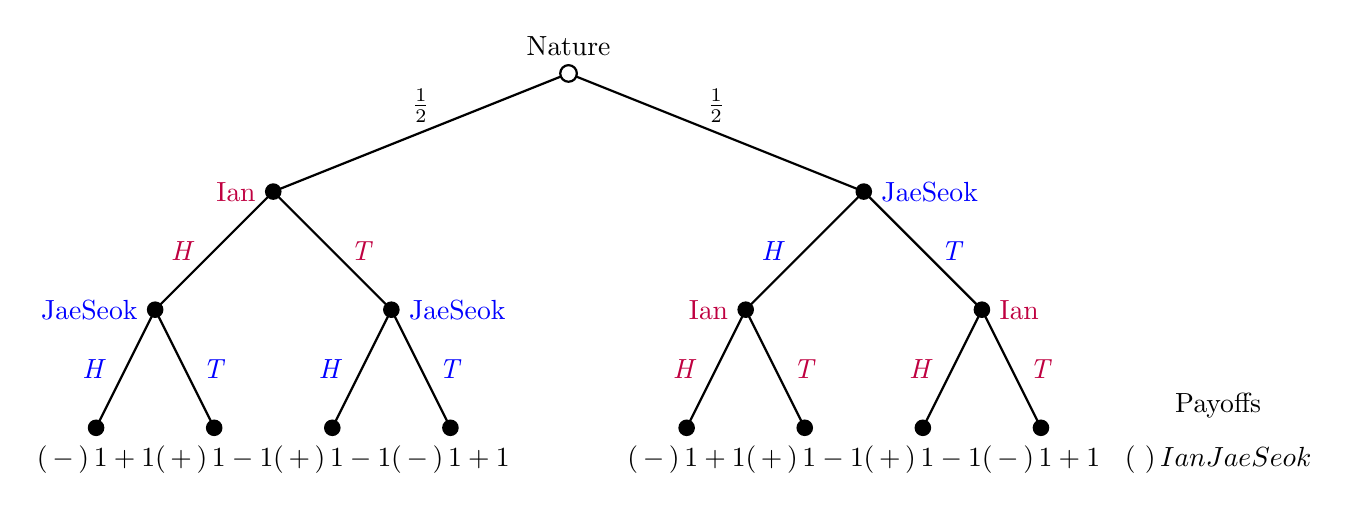
\begin{tikzpicture}[scale=1.5]
        % Nature's move
        \draw[thick] (0,0) -- (-2.5,-1) node[pos=.5,left,above] {$\frac{1}{2}$};
        \draw[thick] (0,0) -- (2.5,-1) node[pos=.5,right,above] {$\frac{1}{2}$};
        % First player's move
        \draw[thick] (-2.5,-1) -- (-3.5,-2) node[pos=.5,left=0.1cm] {\color{purple}\textit{H}};
        \draw[thick] (-2.5,-1) -- (-1.5,-2) node[pos=.5,right=0.1cm] {\color{purple}\textit{T}};
        \draw[thick] (2.5,-1) -- (1.5,-2) node[pos=.5,left=0.1cm] {\color{blue}\textit{H}};
        \draw[thick] (2.5,-1) -- (3.5,-2) node[pos=.5,right=0.1cm] {\color{blue}\textit{T}};
        % Second player's move
        \draw[thick] (-3.5,-2) -- (-4,-3) node[pos=.5,left=0.1cm] {\color{blue}\textit{H}};
        \draw[thick] (-3.5,-2) -- (-3,-3) node[pos=.5,right=0.1cm] {\color{blue}\textit{T}};
        \draw[thick] (-1.5,-2) -- (-2,-3) node[pos=.5,left=0.1cm] {\color{blue}\textit{H}};
        \draw[thick] (-1.5,-2) -- (-1,-3) node[pos=.5,right=0.1cm] {\color{blue}\textit{T}};
        \draw[thick] (1.5,-2) -- (1,-3) node[pos=.5,left=0.1cm] {\color{purple}\textit{H}};
        \draw[thick] (1.5,-2) -- (2,-3) node[pos=.5,right=0.1cm] {\color{purple}\textit{T}};
        \draw[thick] (3.5,-2) -- (3,-3) node[pos=.5,left=0.1cm] {\color{purple}\textit{H}};
        \draw[thick] (3.5,-2) -- (4,-3) node[pos=.5,right=0.1cm] {\color{purple}\textit{T}};
        % Initial and decision nodes
        \draw[fill=white, thick] (0,0) circle[radius=2pt];
        \node[above=0.1cm] at (0,0) {Nature};
        \fill (-2.5,-1) circle (2pt) node[left=0.1cm] {\color{purple}Ian};
        \fill (1.5,-2) circle (2pt) node[left=0.1cm] {\color{purple}Ian};
        \fill (3.5,-2) circle (2pt) node[right=0.1cm] {\color{purple}Ian};
        \fill (2.5,-1) circle (2pt) node[right=0.1cm] {\color{blue}JaeSeok};
        \fill (-3.5,-2) circle (2pt) node[left=0.1cm] {\color{blue}JaeSeok};
        \fill (-1.5,-2) circle (2pt) node[right=0.1cm] {\color{blue}JaeSeok};
        % Terminal nodes
        \fill (-4,-3) circle (2pt) node[below=0.1cm] {$\begin{pmatrix} -1 \\ +1 \end{pmatrix}$};
        \fill (-3,-3) circle (2pt) node[below=0.1cm] {$\begin{pmatrix} +1 \\ -1 \end{pmatrix}$};
        \fill (-2,-3) circle (2pt) node[below=0.1cm] {$\begin{pmatrix} +1 \\ -1 \end{pmatrix}$};
        \fill (-1,-3) circle (2pt) node[below=0.1cm] {$\begin{pmatrix} -1 \\ +1 \end{pmatrix}$};
        \fill (1,-3) circle (2pt) node[below=0.1cm] {$\begin{pmatrix} -1 \\ +1 \end{pmatrix}$};
        \fill (2,-3) circle (2pt) node[below=0.1cm] {$\begin{pmatrix} +1 \\ -1 \end{pmatrix}$};
        \fill (3,-3) circle (2pt) node[below=0.1cm] {$\begin{pmatrix} +1 \\ -1 \end{pmatrix}$};
        \fill (4,-3) circle (2pt) node[below=0.1cm] {$\begin{pmatrix} -1 \\ +1 \end{pmatrix}$};
        % Legend
        \node[above] at (5.5,-3) {Payoffs};
        \node[below=0.1cm] at (5.5,-3) {$\begin{pmatrix} \text{Ian} \\ \text{JaeSeok} \end{pmatrix}$};
    \end{tikzpicture}
\end{figure}